\subsection{Train Accuracy Graphs}

\subsubsection{Learning Rate}

    \begin{figure}[H]
        \minipage{0.5\textwidth}
        
\includegraphics[width=\linewidth]{testsResults/trainAccuracy/def.png}
        \caption{Default settings + learning rate = 0.001}
        \endminipage\hfill
        \minipage{0.5\textwidth}
        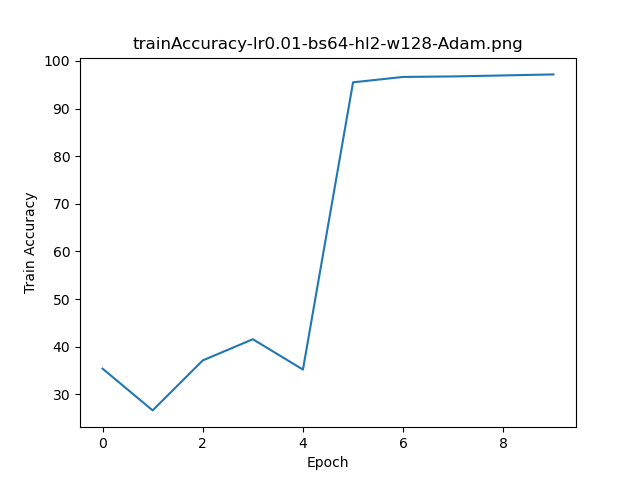
\includegraphics[width=\linewidth]{testsResults/trainAccuracy/trainAccuracy-lr0.01-bs64-hl2-w128-Adam.png}
        \caption{Default settings + learning rate = 0.01}
        \endminipage
    \end{figure}
        \begin{figure}[H]
        \minipage{0.5\textwidth}%
        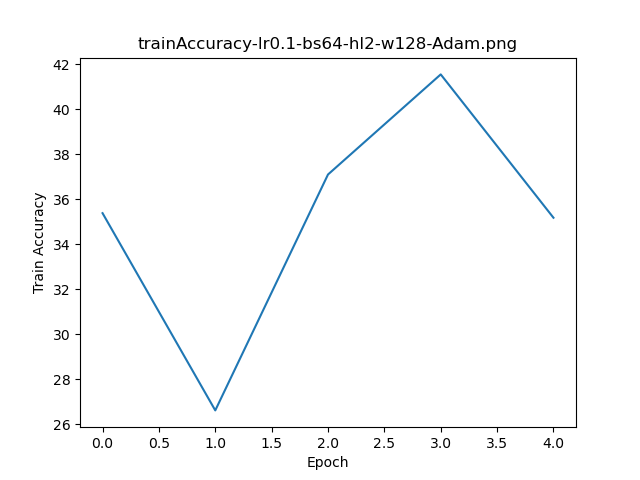
\includegraphics[width=\linewidth]{testsResults/trainAccuracy/trainAccuracy-lr0.1-bs64-hl2-w128-Adam.png}
        \caption{Default settings + learning rate = 0.1}
        \endminipage
    \end{figure}

    \paragraph{Analysis} Making training accuracy smaller than 0.01 seems to be unnecessary for this dataset as it offers little to no improve in accuracy. Setting it to 0.1 on the other hand provides very low accuracy of neural network

\subsubsection{Mini-Batch size}

    \begin{figure}[H]
        \minipage{0.5\textwidth}
        
\includegraphics[width=\linewidth]{testsResults/trainAccuracy/def.png}
        \caption{Default settings + batching size = 64}
        \endminipage\hfill
        \minipage{0.5\textwidth}
        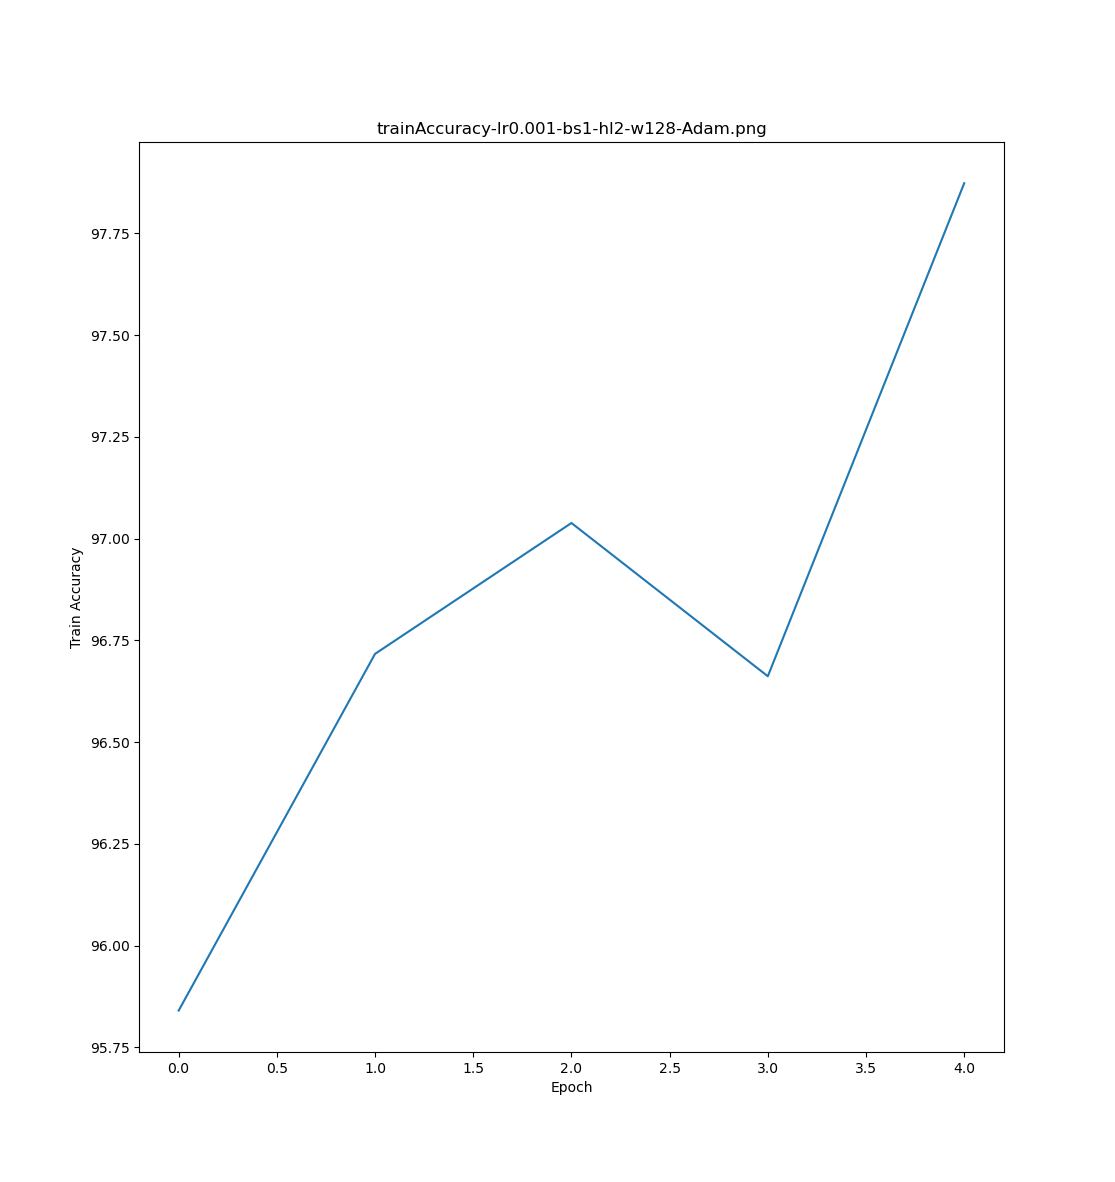
\includegraphics[width=\linewidth]{testsResults/trainAccuracy/trainAccuracy1batch.png}
        \caption{Default settings + batching size = 1}
        \endminipage
    \end{figure}
        \begin{figure}[H]
        \minipage{0.5\textwidth}%
        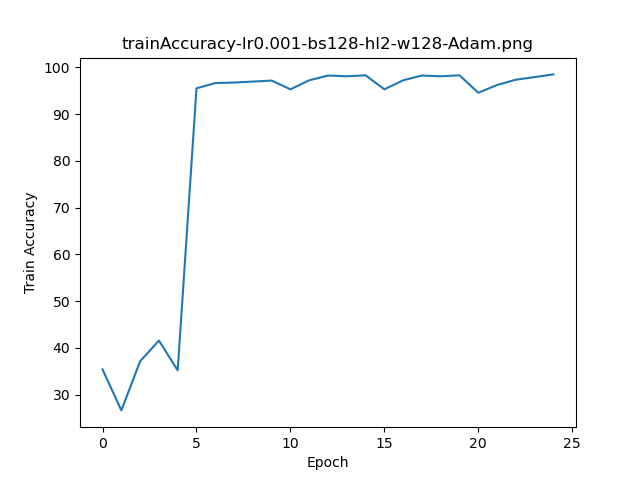
\includegraphics[width=\linewidth]{testsResults/trainAccuracy/trainAccuracy-lr0.001-bs128-hl2-w128-Adam.png}
        \caption{Default settings + batching size = 128}
        \endminipage
        \minipage{0.5\textwidth}%
        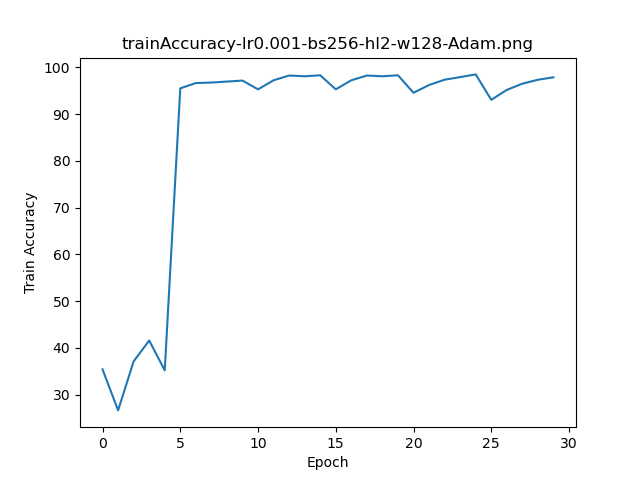
\includegraphics[width=\linewidth]{testsResults/trainAccuracy/trainAccuracy-lr0.001-bs256-hl2-w128-Adam.png}
        \caption{Default settings + batching size = 256}
        \endminipage
    \end{figure}

    \paragraph{Analysis} Increasing batching size does not seem to make drastic change for train accuracy, even setting batching size to 1 offers very good (over 95 \%) accuracy




\subsubsection{Number of Hidden Layers}

    \begin{figure}[H]
        \minipage{0.5\textwidth}
        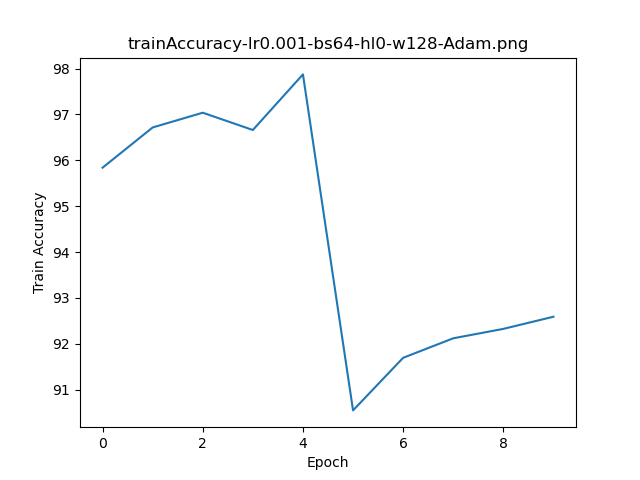
\includegraphics[width=\linewidth]{testsResults/trainAccuracy/trainAccuracy-lr0.001-bs64-hl0-w128-Adam.png}
        \caption{Default settings + hidden layers = 0}
        \endminipage\hfill
        \minipage{0.5\textwidth}
        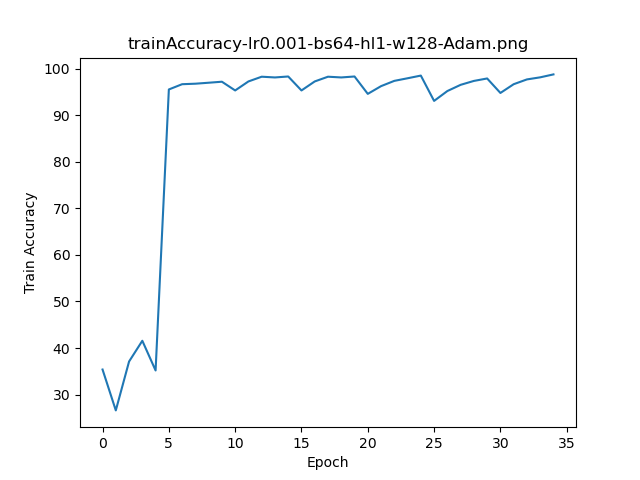
\includegraphics[width=\linewidth]{testsResults/trainAccuracy/trainAccuracy-lr0.001-bs64-hl1-w128-Adam.png}
        \caption{Default settings + hidden layers = 1}
        \endminipage
    \end{figure}
        \begin{figure}[H]
        \minipage{0.5\textwidth}%
        
\includegraphics[width=\linewidth]{testsResults/trainAccuracy/def.png}
        \caption{Default settings + hidden layers = 2}
        \endminipage
        \minipage{0.5\textwidth}%
        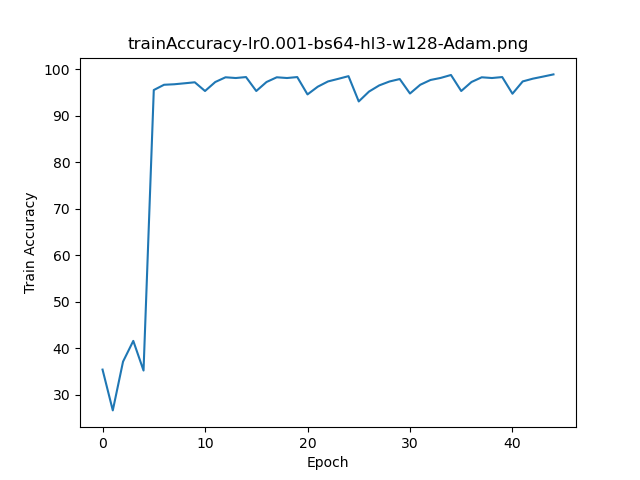
\includegraphics[width=\linewidth]{testsResults/trainAccuracy/trainAccuracy-lr0.001-bs64-hl3-w128-Adam.png}
        \caption{Default settings + hidden layers = 3}
        \endminipage
    \end{figure}

    \paragraph{Analysis} Increasing hidden layers number reduces variety of train accuracy results, with hidden layers set to 0 having accuracy vary between 91 and 98 and with hidden layers equal to 3 showing much smoother graph
\subsubsection{Width}

    \begin{figure}[H]
        \minipage{0.5\textwidth}
        
\includegraphics[width=\linewidth]{testsResults/trainAccuracy/def.png}
        \caption{Default settings + width = 128}
        \endminipage\hfill
        \minipage{0.5\textwidth}
        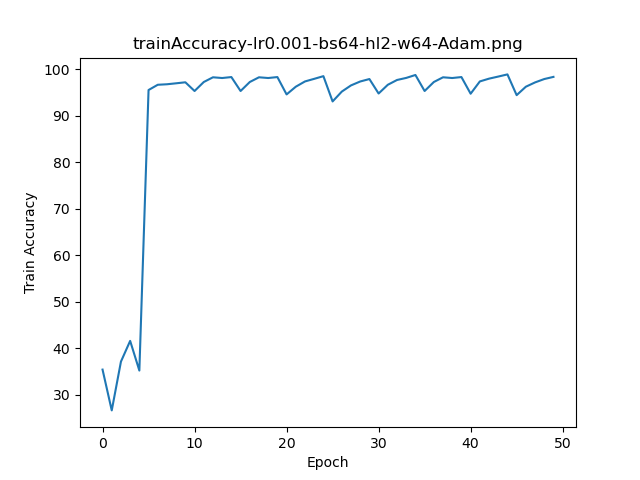
\includegraphics[width=\linewidth]{testsResults/trainAccuracy/trainAccuracy-lr0.001-bs64-hl2-w64-Adam.png}
        \caption{Default settings + width = 64}
        \endminipage
    \end{figure}
        \begin{figure}[H]
        \minipage{0.5\textwidth}%
        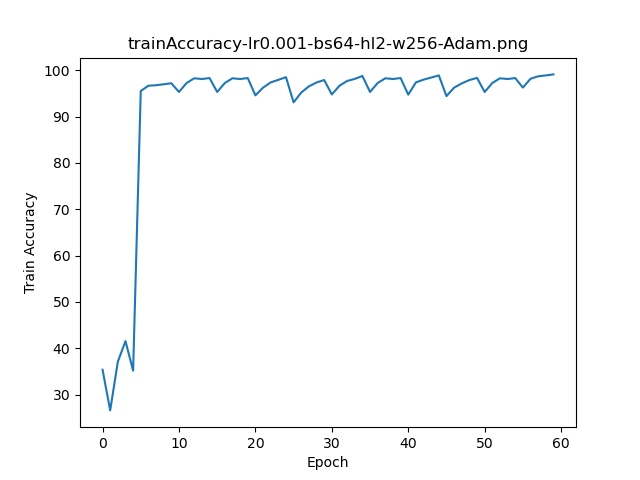
\includegraphics[width=\linewidth]{testsResults/trainAccuracy/trainAccuracy-lr0.001-bs64-hl2-w256-Adam.png}
        \caption{Default settings + width = 256}
        \endminipage
        \minipage{0.5\textwidth}%
        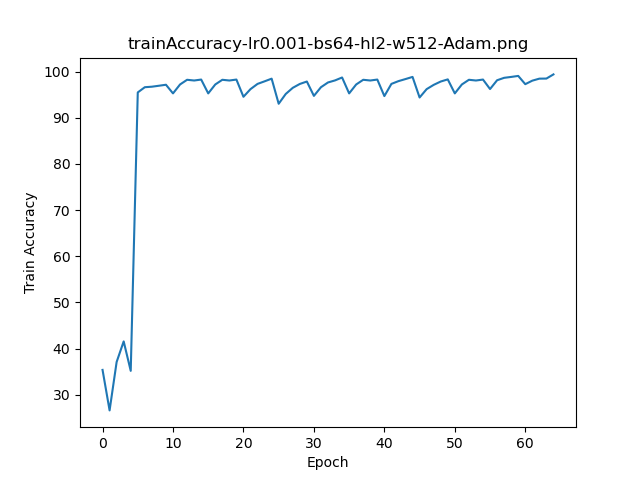
\includegraphics[width=\linewidth]{testsResults/trainAccuracy/trainAccuracy-lr0.001-bs64-hl2-w512-Adam.png}
        \caption{Default settings + width = 512}
        \endminipage
    \end{figure}
    \begin{figure}[H]
        \minipage{0.5\textwidth}%
        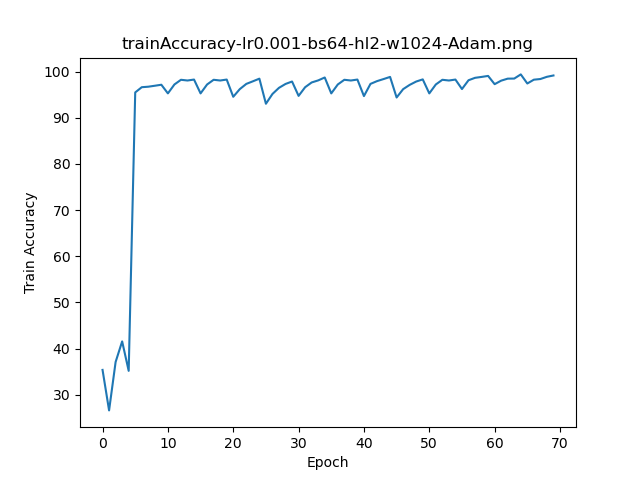
\includegraphics[width=\linewidth]{testsResults/trainAccuracy/trainAccuracy-lr0.001-bs64-hl2-w1024-Adam.png}
        \caption{Default settings + width = 1024}
        \endminipage
    \end{figure}

    \paragraph{Analysis} Changing width does not seem to influence accuracy much

\subsubsection{Optimizer Type}

    \begin{figure}[H]
        \minipage{0.5\textwidth}
        
\includegraphics[width=\linewidth]{testsResults/trainAccuracy/def.png}
        \caption{Default settings + Adam optimizer}
        \endminipage\hfill
        \minipage{0.5\textwidth}
        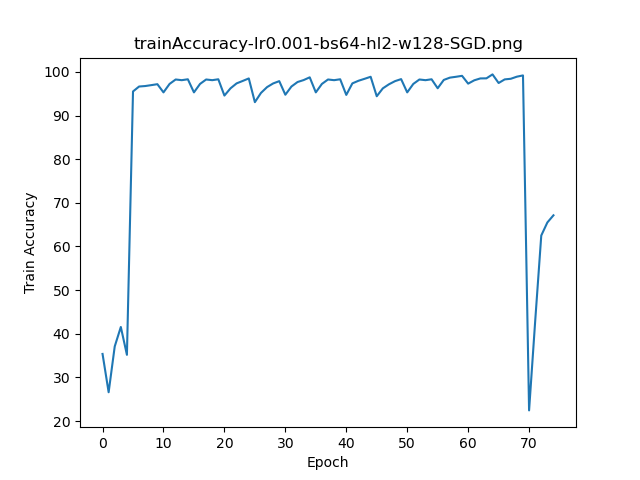
\includegraphics[width=\linewidth]{testsResults/trainAccuracy/trainAccuracy-lr0.001-bs64-hl2-w128-SGD.png}
        \caption{Default settings + learning rate = 0.01}
        \endminipage
    \end{figure}
        \begin{figure}[H]
        \minipage{0.5\textwidth}%
        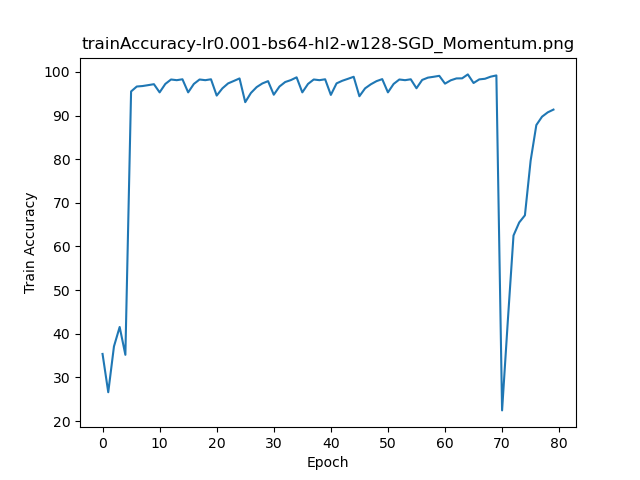
\includegraphics[width=\linewidth]{testsResults/trainAccuracy/trainAccuracy-lr0.001-bs64-hl2-w128-SGD_Momentum.png}
        \caption{Default settings + SGD\_Momentum optimizer}
        \endminipage
    \end{figure}

    \paragraph{Analysis} Changing optimizer type does not seem to influence accuracy much

